% !TEX root = HW4.tex
\newcommand{\spEighteenSvmOneA}{\\
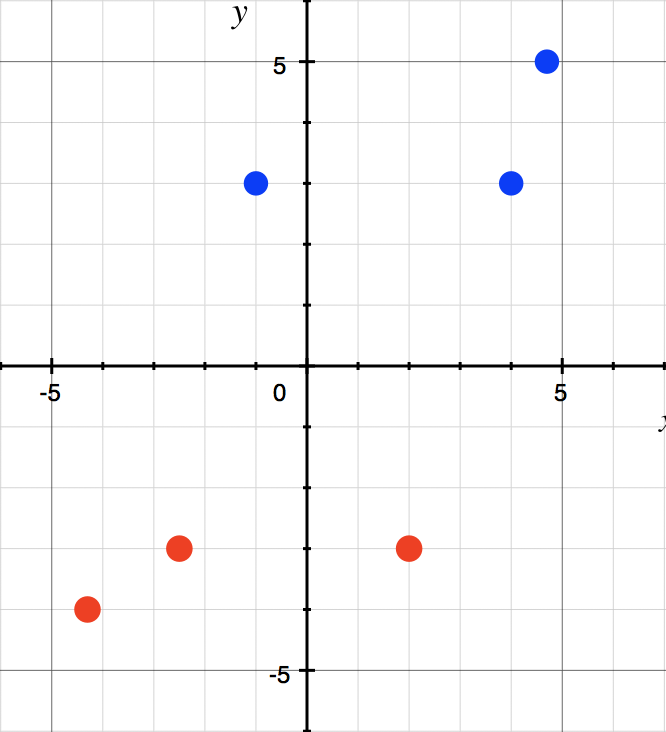
\includegraphics[width=4cm]{1a.png}\\
$\mathbf{w} = [0;\frac{1}{3}]$, $b=0$\\

From the graph its quite clear the $\mathbf{x}_1$ has no effect on the classification. This leaves $\mathbf{w}_2$ and $b$ unknown. We can use the four support vectors to determine the optimal values for these two parameters. We want the decision hyper-plane to be equidistant from each of these vectors which leaves us with $\mathbf{w}_2 = 1$ and $b=0$. $\mathbf{w}_2$ can be further minimized down to $\mathbf{w}_2 = \frac{1}{3}$ to reduce the total cost while conforming the hard SVM constraint. Its important to note that increasing $b$ off of $0$ in either direction requires $\mathbf{w}_2$ to also increase, thereby increasing the total cost. Ex. if $b=\frac{1}{2}$, $\mathbf{w}_2$ would have to be increased to $\frac{1}{2}$, increasing the total cost as mentioned.
}

\newcommand{\spEighteenSvmOneB}{
The support vector are examples: 1, 2, 3, and 5
}

\newcommand{\spEighteenSvmOneC}{
$$
\mathbf{z}=
\begin{bmatrix}
\mathbf{w}_1\\
\mathbf{w}_2\\
b
\end{bmatrix}
P=
\begin{bmatrix}
1 & 0 & 0 \\
0 & 1 & 0 \\
0 & 0 & 0 \\
\end{bmatrix}
\mathbf{q}=
\begin{bmatrix}
0\\
0\\
0
\end{bmatrix}
G=
\begin{bmatrix}
1 & -3 & -1\\
-2.5 & -3 & 1\\
2 & -3 & 1\\
-4.7 & -5 & -1\\
-4 & -3 & -1\\
-4.3 & -4 & 1\\
\end{bmatrix}
\mathbf{h}=
\begin{bmatrix}
-1\\
-1\\
-1\\
-1\\
-1\\
-1\\
\end{bmatrix}
$$
}

\newcommand{\spEighteenSvmOneD}{
When $C=0$ the soft-SVM becomes a hard-SVM and has a margin of 1. If $C=\infty$ the margin is reduced to 0 in order to lower the cost as much as possible.
}

\newcommand{\spEighteenSvmTwoA}{
\begin{align*}
\alpha K_1(\mathbf{x},\mathbf{z}) + \beta K_2(\mathbf{x},\mathbf{z})&=\alpha\Phi(\mathbf{x})^T\Phi(\mathbf{z})+\beta\Phi(\mathbf{x})^T\Phi(\mathbf{z})\\
&=\begin{bmatrix}
\alpha\Phi(\mathbf{x})^T & \beta\Phi(\mathbf{x})^T\\
\end{bmatrix}
\begin{bmatrix}
\alpha\Phi(\mathbf{z}) \\
\beta\Phi(\mathbf{z})
\end{bmatrix} \\
&=(\alpha K_1 + \beta K_2)(\mathbf{x},\mathbf{z}) \\
&=K_3(\mathbf{x},\mathbf{z})
\end{align*}
Which forms a valid kernel function, as the key restriction is that the kernel function must form a proper inner product.
}

\newcommand{\spEighteenSvmTwoB}{
\begin{align*}
K(\mathbf{x},\mathbf{z})
&= (\mathbf{x}^T\mathbf{z})^2 \\
&= (\mathbf{x}_1 \mathbf{z}_1 + \mathbf{x}_2 \mathbf{z}_2)^2 \\
&= (\mathbf{x}_1 \mathbf{z}_1)^2 + 2(\mathbf{x}_1 \mathbf{z}_1)(\mathbf{x}_2 \mathbf{z}_2) + (\mathbf{x}_2 \mathbf{z}_2)^2 \\
&= \mathbf{x}_1^2\mathbf{z}_1^2 + 2\mathbf{x}_1\mathbf{z}_1\mathbf{x}_2\mathbf{z}_2 + \mathbf{x}_2^2\mathbf{z}_2^2 \\
&= \begin{bmatrix}
\mathbf{x}_1^2\\
\sqrt{2}\mathbf{x}_1\mathbf{x}_1\\
\mathbf{x}_2^2\\
\end{bmatrix}^T
\begin{bmatrix}
\mathbf{z}_1^2\\
\sqrt{2}\mathbf{z}_1\mathbf{z}_1\\
\mathbf{z}_2^2\\
\end{bmatrix}\\
\end{align*}

$$
\Phi(\mathbf{x}) = 
\begin{bmatrix}
\mathbf{x}_1^2\\
\sqrt{2}\mathbf{x}_1\mathbf{x}_1\\
\mathbf{x}_2^2\\
\end{bmatrix}
$$
}